\chapter{L'algoritmo}

L'algoritmo implementato consiste in una serie di operazioni che si ripetono ciclicamente, la cui frequenza di esecuzione è regolata da un timer che viene avviato nel momento in cui l'utente attiva l'accordatore.
In questo istante, il programma dà inizio all'operazione di registrazione del suono, che viene realizzata grazie al microfono del calcolatore. 
I passi dell'algoritmo, che vengono eseguiti a ogni scatto del timer, sono i seguenti:
\begin{itemize}
	\item pausa della registrazione,
	\item estrazione del vettore audio dal buffer di registrazione, 
	\item ripresa della registrazione,
	\item calcolo della trasformata discreta di Fourier del segnale audio estratto,
	\item prima stima della frequenza fondamentale realizzata tramite il metodo \emph{Harmonic Product Spectrum}, descritto in \ref{cap:rilevamento_frequenza},
	\item interpolazione dei valori nell'intorno del valore calcolato al fine di aumentare la precisione,
	\item individuazione della frequenza fondamentale a partire dai valori interpolati,
	\item calcolo della differenza tra la frequenza fondamentale e la frequenza di riferimento,
	\item visualizzazione sulla GUI della frequenza fondamentale e della frequenza di riferimento.
\end{itemize}

Di seguito si trova una descrizione dei passi principali dell'algoritmo.

	\section{Rilevamento della frequenza fondamentale}\label{cap:rilevamento_frequenza}
	L'algoritmo utilizzato per rilevare la frequenza fondamentale è l'algoritmo \emph{Harmonic Product Spectrum}, abbreviato dall'acronimo \emph{HPS}.
	Tale metodo sfrutta il fatto che quando viene prodotta una nota con uno strumento musicale, l'energia del suono si concentra principalmente nella frequenza fondamentale e nelle sue armoniche, cioè i suoi multipli interi.

	L'algoritmo HPS moltiplica lo spettro del segnale con un numero \emph{K-1} di versioni differenti dello spettro.
	Le diverse versioni sono ottenute sotto-campionando lo spettro originale con i diversi fattori compresi tra 2 e K.
	La formula \ref{formula:hps_prod} esprime in forma matematica questo passo per un generico spettro X($\omega$) e un generico valore \emph{K}.

		\begin{equation}\label{formula:hps_prod}
			Y(\omega) = \prod_{i=1}^K \left | X(\omega i) \right |
		\end{equation}

	Una volta ottenuto il prodotto Y($\omega$), la frequenza fondamentale viene calcolata come ascissa del massimo della funzione risultante. 
	La formula \ref{formula:hps_max} descrive questo secondo passaggio.

		\begin{equation}\label{formula:hps_max}
			Y_{f0} = \max_{\omega_i} Y \left(\omega_i \right )
		\end{equation}

	In figura \ref{fig:HPS} si può vedere molto chiaramente il funzionamento dell'algoritmo. 
	Dal momento che l'energia è concentrata nelle armoniche, tutte le versioni scalate dei segnali avranno un picco nella frequenza fondamentale. 
	L'ampiezza del prodotto in tale frequenza, perciò, risulta essere molto elevata.
	Ciò non si verifica con le altre armoniche.
	A causa delle diverse scalature, infatti, il prodotto per questi valori di frequenza è il risultato tra valori di picco e valori molto bassi.
	Ciò comporta una riduzione del valore del prodotto per tali frequenze. 
	La funzione prodotto si può vedere nella parte destra della figura. 
	Il segnale risultante presenta un unico picco nella frequenza fondamentale.
	A questo punto, quindi, una semplice operazione di ricerca del massimo risulta essere sufficiente per trovare la frequenza fondamentale \cite{Cuadra01efficientpitch}.

		\begin{figure}[h]
		  \begin{center} 
		    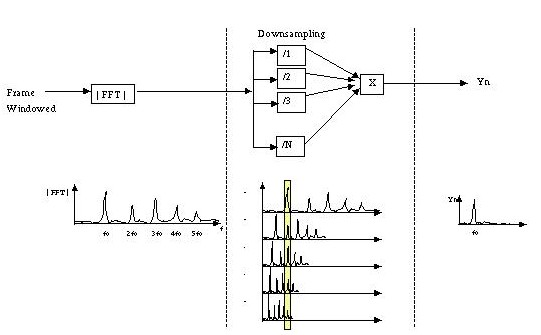
\includegraphics[width=\textwidth*\real{0.68}]{images/ch_04/processo.jpg}
		  \end{center} 
		  \caption{\textit{Metodo HPS}}  
		  \label{fig:HPS}
		\end{figure}

	Nel contesto dell'accordatore, il metodo è stato applicato moltiplicando il segnale originale con le prime quattro versioni scalate del segnale.
	Ciò è stato possibile dal momento che la frequenza del segnale ottenuto risulta essere maggiore della frequenza più alta delle corde della chitarra, cioè 329.63 hz.
	La frequenza massima del prodotto tra i segnali, infatti, si ottiene dividendo la frequenza massima del segnale originale per il fattore massimo di scala.
	Sostituendo i valori 4000 hz e 5, il risultato che si ottiene è 800 hz, che è ben oltre il doppio dell'ottava della nota più acuta suonata dalla chitarra. L'operazione di scalatura, quindi, non compromette in alcun modo la ricerca della frequenza fondamentale.

	L'algoritmo, inoltre, prevede di usare la tecnica di zero-padding sui segnali scalati in modo che essi vengano adattati alla lunghezza del vettore originale. 
	Questa operazione è stata evitata troncando tutte le versioni dei vettori scalate al numero di elementi del vettore più corto.
	Per quanto detto precedentemente, questa operazione non lede la generalità dell'algoritmo.

	L'operazione di ricerca del massimo è calcolata su una versione ulteriormente finestrata della funzione prodotto. 
	In particolare, vengono escluse le frequenze inferiori ai 40 hz in quanto il rumore in questo range è molto intenso, come discusso nel capitolo \ref{cap:rumore}.
	La generalità dell'algoritmo di ricerca della frequenza non viene lesa da questa operazione, in quanto la frequenza fondamentale minore tra le note della chitarra è di 82.41 hz.

	Il risultato del doppio finestramento può essere paragonato all'applicazione di un filtro passa-banda ideale sul segnale prodotto, con intervallo di frequenze pari a [40,800] hz.
	Si è potuto utilizzare un filtro ideale in quanto tutte le operazioni effettuate riguardano il dominio delle frequenze.
	Il segnale nel dominio del tempo, quindi, non deve essere ricostruito.




